\documentclass[9pt]{beamer}

%!TEX root = ../notas_de_clase.tex

%preamble

%language
\usepackage[spanish,es-nodecimaldot]{babel}
\usepackage[utf8]{inputenc}
\usepackage{apacite}
\usepackage[absolute,overlay]{textpos}

%packages
\usepackage[Algoritmo]{algorithm}
\usepackage{algorithmicx}
\usepackage[noend]{algpseudocode}
\usepackage{mathtools}
\setlength {\marginparwidth}{2cm}
\usepackage{todonotes}
\usepackage{amsbsy}
\usepackage{amssymb}
\usepackage{amsmath,bm}
\usepackage{dsfont}

\usepackage{xcolor}
\providecommand{\sred}[1]{\textcolor{red}{#1}}
\providecommand{\sblue}[1]{\textcolor{blue}{#1}}
\providecommand{\red}[1]{\textcolor{red}{\text{#1}}}
\providecommand{\blue}[1]{\textcolor{blue}{\text{#1}}}
\providecommand{\redb}[1]{\textcolor{red}{\textbf{#1}}}
\providecommand{\blueb}[1]{\textcolor{blue}{\textbf{#1}}}
\usepackage{graphicx}
\usepackage{fancybox}
\usepackage{booktabs}
\usepackage{caption}
\usepackage{float}
%\usepackage[longend,ruled,algochapter,linesnumbered,lined,boxed,commentsnumbered,spanish]{algorithm2e}
%\usepackage[algo2e]{algorithm2e}
\usepackage{amssymb}
\usepackage{amstext}
\usepackage{bm}
\usepackage{wrapfig}
\usepackage{subcaption} % para_unsupervised_chapter

%formatting

\usepackage[export]{adjustbox}

%caption para figuras
\captionsetup[figure]{width=.8\linewidth, font=small,labelfont={bf},name={Fig.},labelsep=period}
\captionsetup[table]{width=.8\linewidth,font=small,labelfont={bf},name={Tabla},labelsep=period}



\ifx\byn\undefined
    \definecolor{my_blue}{HTML}{C2D5FF}
    \definecolor{my_red}{HTML}{FFC2C2}
    \definecolor{my_yellow}{HTML}{FFFFE0}
\else
    \definecolor{my_blue}{HTML}{FFFFFF}
    \definecolor{my_red}{HTML}{FFFFFF}
    \definecolor{my_yellow}{HTML}{FFFFFF}
\fi


\usepackage[framemethod=TikZ]{mdframed}
\mdfdefinestyle{discusion}{%
    %linecolor=black,
    %outerlinewidth=0pt,
    roundcorner=0pt,
    innertopmargin=5pt,
    innerbottommargin=5pt,
    innerrightmargin=20pt,
    innerleftmargin=20pt,
    backgroundcolor=my_blue}

\colorlet{Green}{green!90}


\mdfdefinestyle{ejemplo}{%
    %linecolor=black,
    %outerlinewidth=0pt,
    roundcorner=0pt,
    innertopmargin=5pt,
    innerbottommargin=5pt,
    innerrightmargin=20pt,
    innerleftmargin=20pt,
    backgroundcolor=my_yellow}


\mdfdefinestyle{pendiente}{%
    style = discusion, 
    backgroundcolor=my_red}


\RequirePackage{url}



%definitions
\def\td{{\text d}}
\def\cN{{\mathcal N}}
\def\cX{{\mathcal X}} 
\def\cC{{\mathcal C}} 
\def\N{{\mathbb N}}
\def\d{{\text d}}
\def\datos{{\mathcal D}}
\def\eye{{\mathbb I}}
\def\ssum{{\scriptstyle\sum}}
\def\bepsilon{{\bm \epsilon}}
\def\tx{\tilde{x}}
\def\tX{\tilde{X}}
\def\thetaMAP{\theta_\text{MAP}}
\newcommand{\gp}{\ensuremath{\mathcal{GP}}}
\newcommand{\pr}{\ensuremath{\mathbb{P}}}
\newcommand{\x}{\ensuremath{\mathbf{x}}}
\newcommand{\z}{\ensuremath{\mathbf{z}}}
\newcommand{\cvector}{\ensuremath{\mathbf{c}}}
\newcommand{\e}{\ensuremath{\mathbf{e}}}
\newcommand{\y}{\ensuremath{\mathbf{y}}}
\newcommand{\bx}{\ensuremath{\textcolor{blue}{X}}}
\newcommand{\by}{\ensuremath{\textcolor{blue}{Y}}}
\newcommand{\rx}{\ensuremath{\textcolor{red}{X_*}}}

\newcommand{\R}{\mathbb{R}}
\newcommand{\norm}[1]{\left\lVert#1\right\rVert}




\DeclareMathOperator*{\argmax}{arg\,max}
\DeclareMathOperator*{\argmin}{arg\,min}
\DeclareMathOperator{\E}{\mathbb{E}}
\DeclareMathOperator{\V}{\mathbb{V}}
\DeclareMathOperator{\KL}{\text{KL}}
\DeclareMathOperator{\MVN}{\text{MVN}}
\newcommand\deq{\stackrel{\mathclap{\normalfont\mbox{\tiny def}}}{=}}
%\newcommand{\E}[1]{\mathbb E \left[#1\right]}
\newcommand{\trace}[1]{\text{Tr} \left[#1\right]}


\usepackage{amsthm}

%-------------------------------------------
% Newtheorem
%-------------------------------------------
\newtheorem{axioma}{\textcolor{red}{Axioma}}
\newtheorem{definicion}{Definición}
\newtheorem*{notacion}{Notación}
\newtheorem{teorema}{Teorema}
\newtheorem{corolario}{Corolario}
\newtheorem{lema}{Lema}
\newtheorem{lemaZ}{\textcolor{red}{Lema}}
\newtheorem{propiedad}{Propiedad:}
\newtheorem{proposicion}{Proposición:}
\newtheorem*{observacion}{Observación}
\newtheorem*{comentario}{Comentario}
\newtheorem*{ejemplo}{Ejemplo}
\newtheorem*{resultado}{Resultado}
\newtheorem*{propuesto}{Ejercicio propuesto}
\newtheorem*{demostracion}{Demostración} % No se usa, usar \begin{proof}\end{proof} que son por default.

%listing paackage para código
\usepackage{listings}
\usepackage{xcolor}
 
\definecolor{codegreen}{rgb}{0,0.6,0}
\definecolor{codegray}{rgb}{0.5,0.5,0.5}
\definecolor{codepurple}{rgb}{0.58,0,0.82}
\definecolor{backcolour}{rgb}{0.95,0.95,0.92}
 
\lstdefinestyle{mystyle}{
    xleftmargin=0.15\textwidth,
    linewidth=0.8\textwidth,
    backgroundcolor=\color{backcolour},   
    commentstyle=\color{codegreen},
    keywordstyle=\color{magenta},
    numberstyle=\tiny\color{codegray},
    stringstyle=\color{codepurple},
    basicstyle=\ttfamily\footnotesize,
    breakatwhitespace=true,         
    breaklines=true,                 
    captionpos=b,                    
    keepspaces=true,                 
    numbers=left,                    
    numbersep=5pt,                  
    showspaces=false,                
    showstringspaces=false,
    showtabs=false,                  
    tabsize=2
}
 
\lstset{style=mystyle}

\numberwithin{equation}{section}

\usetheme{simple}

\title{Clase 8 - Clasificación (parte 1)}
\subtitle{Aprendizaje de Máquinas - MA5204}
\date{\today}
\author{Felipe Tobar} 
\titlegraphic{
\begin{figure}[htp] 
    \centering
        
\includegraphics[width=0.15\textwidth]{../img/Uchile.pdf}% 
\end{figure}
}
\institute{Department of Mathematical Engineering \&\\ Center for Mathematical Modelling\\Universidad de Chile}

\begin{document}
\begin{frame}
  \titlepage
\end{frame}

\section{Problema de Clasificación}
\begin{frame}{Introducción - Problema de Clasificación}
El problema de clasificación dice relación con la identificación del conjunto, categoría o \emph{clase} a la cual pertenece un elemento en base a sus \emph{características}. \vspace{0.5cm} \pause

\begin{columns}

  \begin{column}{0.5\textwidth}
    En el contexto del aprendizaje supervisado, puede ser visto como un problema de regresión. \vspace{0.5cm} \pause

    En efecto, basta suponer que $y$ variable de salida (o variable dependiente) es \emph{categórica} y usualmente denotada por $\{ 0 , 1 \}$ en el caso binario o para el caso multiclase $\{ 1 \dots K \}$ \vspace{0.5cm} \pause

    Entre los métodos de clasificación existentes, trabajaremos en 

    \begin{enumerate}
      \item \emph{k} vecinos más cercanos \pause
      \item Regresión Logística \pause
      \item Support Vector Machines (SVM) \pause

    \end{enumerate}


  \end{column}

  \begin{column}{0.5\textwidth}
    \centering
    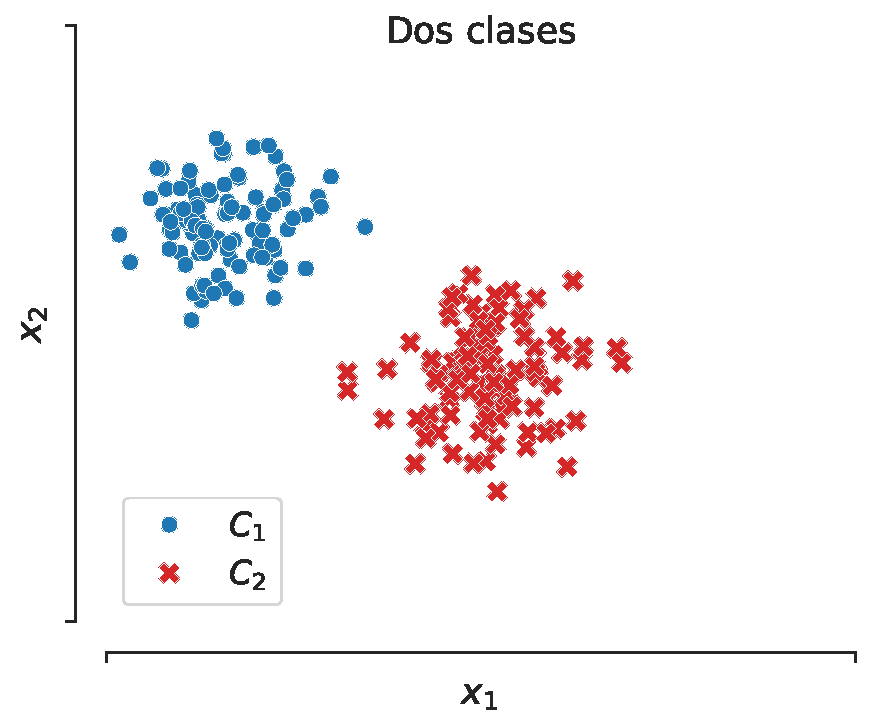
\includegraphics[width=5cm]{../img/cap3_dosclases.pdf}\\
    \captionof{figure}{Ejemplo del problema  de clasificación binaria, donde la clase $\cC_1$ está presentada en azul y la clase $\cC_2$ en rojo.}
    \label{fig:puntos_2d}
  \end{column}


\end{columns}


\end{frame}

\section{Clasificación Lineal}

\begin{frame}{Clasificación Lineal - Binaria}

Consideremos el caso binario K=2 clases, proponemos un modelo lineal para relacionar la variable independiente con su clase, es decir, $y(x) = a^Tx+b$ tal que  $x \in \cC_1$ si $y(x) \geq 0$, en caso contrario,  $x \in \cC_2$. \pause

Para encontrar los parámetros $a,b$ óptimos, sean $x_1$ y $x_2$ en la región de decisión $y(x)=0$ \pause  
\begin{align*}
  0 &= y(x_1) - y(x_2) \nonumber\\ 
    &= a^\top x_1 + b - a^\top x_2 - b \nonumber\\ 
    &= a^\top (x_1-x_2).
\end{align*}
\pause
Además, observemos que para cualquier $x$ en la región de decisión se tiene que 
\begin{equation*}
  \norm{\text{proy}_a(x)} = \norm{x}cos(\theta) = \norm{x} \frac{a^\top x}{\norm{a}\cdot\norm{x}} = -\frac{b}{\norm{a}}
\end{equation*}

Con lo que tenemos una intepretación geométrica de ambos parámetros. 

\end{frame}

\begin{frame}{Clasificación Lineal - Binaria}

\begin{figure}[h]
    \centering
    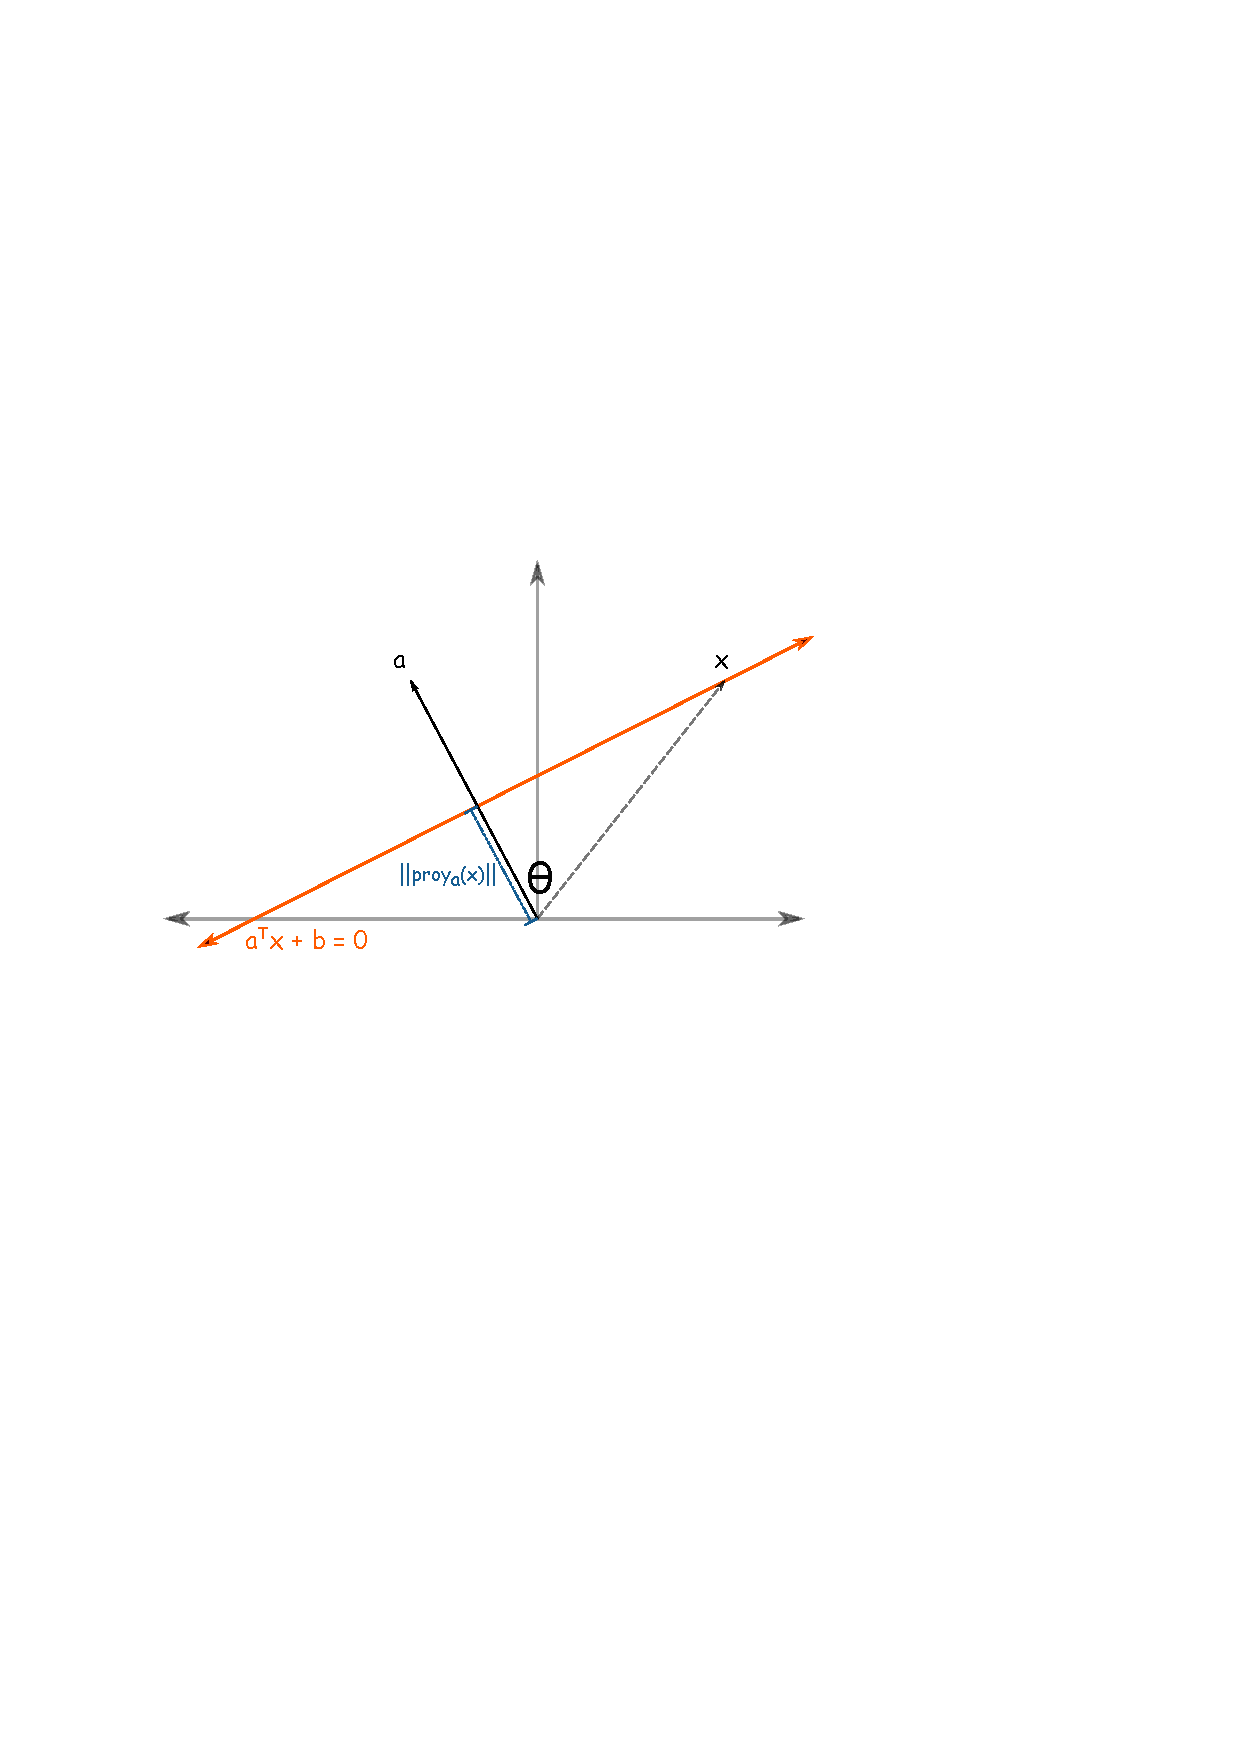
\includegraphics[width=0.5\textwidth]{../img/cap3_proy.pdf}
    \caption{Proyección de un punto sobre la región de decisión. }
\end{figure}


\end{frame}

\begin{frame}{Clasificación Lineal - Binaria}

También es posible interpretar $y(x)$ como una distancia con signo entre un $x\in\R^M$ cualquiera y la superficie de decisión. \pause

Para ver esto, consideremos $x\in\R^M$ y descompongámoslo en dos componentes: la primera denotada por $x_{\bot}$, la cual es la proyección ortogonal de $x$ en el hiperplano de  decisión, y la segunda que es perpendicular al hiperplano (y consecuentemente paralela al vector $a$) denotada por $r\frac{a}{\left \| a \right \|}$, donde $r$ denota la distancia (positiva o negativa) entre $x$ y el  hiperplano de  decisión. Expresamos entonces  \pause

\begin{equation*}
  x = x_{\bot}+r\frac{a}{\left \| a \right \|},
\end{equation*}

y observamos que \pause

\begin{equation*}
  y(x) 
  = a^\top x+b 
  =a^\top  \left( x_{\bot} + r\frac{a}{\left \| a \right \|} \right) +b 
  = \underbrace{a^\top x_{\bot} +b }_{=0} +   r\frac{a^\top  a}{\left \| a \right \|}
  = r||a||.
\end{equation*}

\pause 

Luego $r = \frac{y(x)}{\norm{a}}$ y como $r$ es una medida con signo, $y(x)$ también lo es. 


\end{frame}

\begin{frame}{Clasificación Lineal - Múltiples clases}

El caso de múltiples clases ($K>2$) puede ser enfrentado mediante una extensión del caso binario, algunas de ellas 

\begin{enumerate}

  \item \textbf{One versus rest: } Construcción de $K-1$ clasificadores binarios que discrimina una clase $\cC_k$ del resto \pause


  \item \textbf{One versus one: } Construccion de $K(K-1)/2$ clasificadores binarios que discriminan entre cada par posible de clases \pause

\end{enumerate}

\textbf{¿Qué problema presentan estos métodos?} \pause Busquemos otra forma \pause 

\vspace{0.5cm}

Una alternativa más robusta para resolver el problema de clasificación multiclase es construir un clasificador para $K$ clases que contiene $K$ funciones lineales de la forma 
\begin{equation*}
  y_k(x) = a_k^\top x + b_k, \quad k=1,\ldots,K.
\end{equation*}
\pause 
Donde $x$ es asignado a la clase $\mathcal{C}_k$ si y solo si $y_k(x) > y_j(x), \forall j\neq k$, es decir: 

\begin{equation*}
  \mathcal{C}(x) = \underset{k}{\argmax}\hspace{1mm} y_j(x).
\end{equation*}

\pause 
\textbf{¿Qué ventajas posee este método?}

\end{frame}

\section{Ajuste mediante mínimos cuadrados}

\begin{frame}{Ajuste mediante mínimos cuadrados}

Ya hemos planteado el modelo y analizado el rol  y significado de cada uno de sus parámetros; ahora queda por estudiar cómo determinar dichos parámetros $a$ y $b$, dado un conjunto de datos $\datos$.
\newline \pause 
Consideremos el  punto $x\in\R^M$ con clase $c\in\{\mathcal{C}_k\}_{k=1}^K$. Usaremos la \emph{codificación} $t \in\{0,1\}^K$ para representar la pertenencia de $x$ a su respectiva clase. Es decir, \pause
\begin{equation*}
  c = \cC_j \Leftrightarrow [t]_j=1 \wedge [t]_i=0, \quad \forall i\neq j.
\end{equation*}
Este tipo de codificación  es conocida como \emph{one-hot  encoding.} \textbf{¿Por qué la usamos?} \pause \newline
Asumiendo entonces un modelo lineal para cada clase $\mathcal{C}_k$, se tiene que
\begin{equation*}
  y_k(x) = a_k^\top x + b_k = \tilde{\theta}_k^\top\tx, \quad \text{donde } \tx = \left( \begin{matrix} x\\ 1 \end{matrix}\right)\in\R^{M+1} ,\quad
  \tilde{\theta}_k = \left( \begin{matrix} a_k\\ b_k \end{matrix}\right)\in\R^{M+1}
\end{equation*}
\newline \pause
Lo anterior se puede unir en un único sistema matricial:

\begin{equation*}
\tilde{\Theta} = \left(\theta_1,\cdots,\theta_K\right)\in\R^{(M+1)\times K} \implies  y(x) = \left( \begin{matrix}y_1(x) \\\vdots \\ y_K(x) \end{matrix}\right) = \tilde{\Theta}^\top \tilde{x}.
  \end{equation*}




\end{frame}

\begin{frame}{Ajuste mediante mínimos cuadrados}
Con la notación establecida, ahora podemos enfocarnos en el entrenamiento del modelo.  Para esto consideremos un conjunto de entrenamiento $\{(x_n,t_n)\}_{n=1}^N$. El enfoque de entrenamiento será el correspondiente a mínimos cuadrados asociado al error de asignación:

\begin{equation*}
  J = \sum_{i=1}^N \norm{t_i - \tilde{\Theta}^\top\tx_i}_2^2
\end{equation*}  \pause

Por otra parte, definiendo las siguientes matrices:

\begin{equation*}
  T = \left(\begin{matrix}
    t_1^\top\\
    \vdots\\
    t_N^\top
  \end{matrix}\right)\in\R^{N\times K},\qquad
  \tX = \left(\begin{matrix}
    t_1^\top\\
    \vdots\\
    t_N^\top
  \end{matrix}\right)\in\R^{N\times (M+1)}
\end{equation*}

\pause

se tiene el siguiente resultado:

\end{frame}

\begin{frame}{Ajuste mediante mínimos cuadrados}

\begin{lemma}
  Bajo la notación anterior, $J=\operatorfont{Tr} \left((\tX\tilde{\Theta}-T)^\top (\tX\tilde{\Theta}-T)\right)$ y su mínimo es alcanzado en: 
  \begin{equation*}
    \tilde{\Theta} = (\tilde{X}^\top\tilde{X})^{-1}\tilde{X}^\top T
  \end{equation*}
  donde $\operatorfont{Tr}$ corresponde al operador traza: $A\in\R^{n\times n}\mapsto \operatorfont{Tr}(A):=\sum\limits_{i=1}^n a_{ii}$.
\end{lemma}


\end{frame}

\begin{frame}{Ajuste mediante mínimos cuadrados}

\begin{proof}
\begin{align*}
  J &= \sum_{i=1}^N \norm{t_i - \tilde{\Theta}^\top\tx_i}_2^2 = \sum_{i=1}^N \norm{\left(T - \tX\tilde{\Theta}\right)_{i\cdot}}_2^2 = \sum_{i=1}^N \sum_{j=1}^K \left(T - \tX\tilde{\Theta}\right)_{ij} \left(T - \tX\tilde{\Theta}\right)_{ij}\\
  &= \sum_{i=1}^N \sum_{j=1}^K \left(T - \tX\tilde{\Theta}\right)^\top_{ji} \left(T - \tX\tilde{\Theta}\right)_{ij} =  \sum_{j=1}^K \left[\left(T - \tX\tilde{\Theta}\right)^\top \left(T - \tX\tilde{\Theta}\right)\right]_{jj}\\
  &=\operatorfont{Tr} \left((\tX\tilde{\Theta}-T)^\top (\tX\tilde{\Theta}-T)\right).
\end{align*}
  
Por otra parte:
\begin{equation*}
  \frac{\partial J}{\partial\tilde{\Theta}} = 2(\tX\tilde{\Theta}-T)^\top\tX=0 \iff \tilde{\Theta}^\top\tX^\top\tX - T^\top\tX = 0 
\end{equation*}
\begin{equation*}
\iff \tilde{\Theta}^\top = T^\top\tX(\tX^\top\tX)^{-1}\iff \tilde{\Theta} = (\tX^\top\tX)^{-1}\tX^\top T
\end{equation*}
  
Y dado que $J$ es estrictamente convexo, su mínimo se alcanza en su único punto crítico.  

\end{proof}


\end{frame}

\begin{frame}{Ajuste mediante mínimos cuadrados}
Problemáticas conceptuales de este enfoque: 
\begin{enumerate}
  \item Sensibilidad a presencia de puntos aislados (outliers) \pause
  \item Intervención ''manual'' de las etiquetas \pause
\end{enumerate}
\begin{figure}[H]
  \centering
  \visible<3->{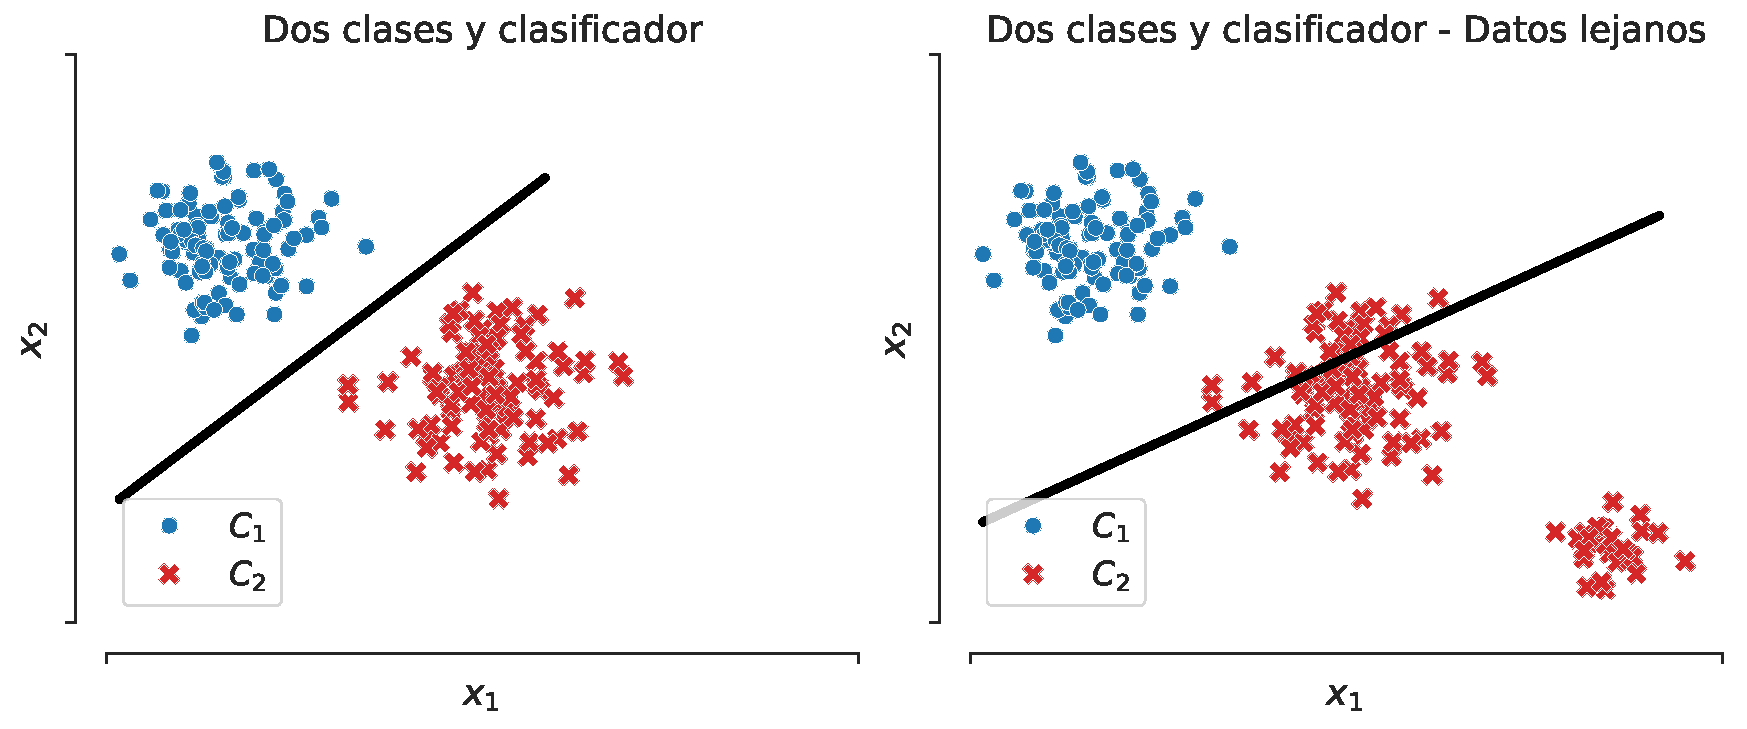
\includegraphics[width=0.8\textwidth]{../img/cap3_dosclases_clasificador.pdf}}\\
  \caption{Ejemplo ilustrativo sobre cómo los puntos lejanos de una clase pueden afectar incorrectamente los resultados.}
  \label{fig:clasif_mse}
\end{figure}


\end{frame}

\begin{frame}
  \titlepage
\end{frame}



%Quitar de comentarios apenas se agregue alguna referencia 
%\bibliography{../capitulos/referencias} %Bibliografía
%\bibliographystyle{apacite}
\end{document} 